\documentclass[a4paper,12pt]{llncs}
\usepackage[top=25mm, bottom=25mm, left=25mm, right=25mm]{geometry}

\usepackage{times}
\usepackage{comment} 
\usepackage{amsmath} 
\usepackage{amssymb}
\usepackage{graphicx,subfigure}
\usepackage{epsfig}
\usepackage{url}
\usepackage{caption}
\usepackage{cite}
\usepackage{comment}

%\usepackage{enumitem}
%\usepackage{wrapfig}

%\usepackage{listings}
%\usepackage{color}
%\usepackage{soul,color}


%\usepackage{enumitem}
%\usepackage[noend]{algorithmic}
%\usepackage{algorithm}
%\usepackage{verbatim}
%\usepackage[noend]{algpseudocode}

%\usepackage[table,xcdraw]{xcolor}
%\usepackage[noend]{algpseudocode}
%\usepackage[ruled,linesnumbered,vlined]{algorithm2e}

%\newfloat{program}{thp}{lop} 
%\floatname{program}{Program}
\newcommand{\ie}{i.e.} 
\newcommand{\eg}{e.g.} 
\newcommand{\et}{et al. }
\newtheorem{mydef}{Example}
\newtheorem{mytheorem}{Theorem}
\newtheorem{myproof}{Proof}
\renewcommand{\labelitemi}{\scriptsize$\blacksquare$} 

\begin{document}

\title{Cluster-based Data Generator}

%\author{ Xiufeng Liu }
%\institute{Technical University of Denmark\\
%\email{\{xiuli\}@dtu.dk}
%}

\maketitle

\begin{abstract}
\end{abstract}


\section{The Data Generator}
Recall from Section 3 that the proposed benchmark requires n time series as input,
each corresponding to an electricity consumer. Testing the scalability of a system therefore requires running the benchmark with increasing values of $n$. Since it is difficult to obtain large amounts of smart meter data due to privacy issues, and since using randomly-generated time series may not give accurate results, we propose a data generator for realistic smart meter data. 


\section{Generator design}
The intuition behind the data generator is as follows. Since electricity consumption depends on external temperature and daily activity, we start with a small seed of real data and we generate the daily activity profiles (recall Figure 3) and temperature regression lines (recall Figure 2) for each consumer therein. To generate a new time series, we take the daily activity pattern from a randomly-selected consumer in the
real data set, the temperature dependency from another randomly-selected consumer, and we add some white noise. Thus, we first disaggregate the consumption time series of existing consumers in the seed data set, and we then re-aggregate the different pieces in a new way to create a new consumer. This gives us a realistic new consumer whose electricity usage combines the characteristics of multiple existing consumers.


\begin{figure}[htp]
\centering
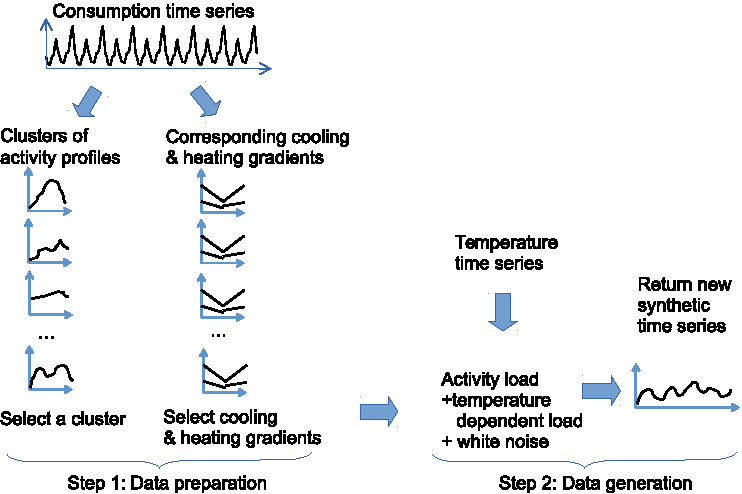
\includegraphics[width=0.7\textwidth]{images/datagenoverview}
\caption{Illustration of the proposed data generator.}
\label{fig:datagenoverview}
\end{figure}



Figure~\ref{fig:datagenoverview} illustrates the proposed data generator. As the data preparation step, we use the PAR algorithm from [Espinoza et al. 2005] to generate daily load profile for each consumer in the seed data set. We then run the k-means clustering algorithm (for some specified value of k, the number of clusters) to group consumers with similar daily load profiles. We also run the 3-line algorithm and record the heating and cooling gradients for each consumer. We now create a new time series proceed as the following details. We randomly select a cluster, and randomly select a daily activity load profile from the chosen cluster. Next, we randomly select a three-line model among the other customers in the chosen cluster. We then input a temperature time series \footnote{In our experiments, we used the temperature time series corresponding to the southern-Ontario city from which we obtained the real data set.}. Now we have all the parameters needed for generating a new time series. 

An hourly consumption measurement of a daily load is generated by the formula:
\begin{equation}
y^* = y_{a}   + y_t  + \epsilon
\end{equation}
where $ y_{a}$ is the activity load at a given hour; $y_t$ is the temperature-dependent load computed by the simple linear regression function with the temperature $t$ and the three-line model (see Figure~\ref{fig:genthreeline});
\begin{equation}
y_t = 
\begin{cases}
 \beta_0t + b_0 & \text{ if } t < t_0  \\ 
\beta_1t + b_1 & \text{ if } t_0 \leq t < t_1 \\ 
\beta_2t + b_2 & \text{ if } t_1 \leq t 
\end{cases}
\end{equation}
and $\epsilon$ is Gaussian white noise component with some specified standard deviation $\delta$. 

\begin{figure}[t]
\centering
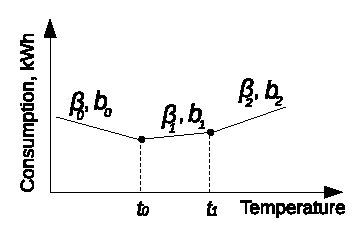
\includegraphics[scale=0.8]{images/genthreeline}
\caption{A three-line model}
\label{fig:genthreeline} 
\end{figure}




\section{Implementation}
The data generator is implemented as two modules. One module is for parameter preparation, and the other module is for data generation. They both are implemented in Spark in order for large-scale data generation. In the parameter preparation step, first we compute the activity load of each customer in a seed data set by stripping the impact by weather temperature, which uses the PAR algorithm. Second, we compute the daily load profile of each customer based on the resulted activity load time series by the statistic method, \ie, compute the mean and the standard deviation at each hour of the day. Third, we do the $k$-mean clustering on the generated daily activity load profiles of all customers with a given value for $k$. In addition, we  compute the heating and cooling gradients of each customer in the seed data set using the three-line algorithm. In the end, we get the  output from the first step, including clustered daily load profiles, the standard deviations, heating and cooling gradients of all the customers in the seed data set. The first step is the parameter preparation process using a particular seeded data, which only needs to run once. The parameters can be re-used. The performance is, therefore, not important. The second step is data generation process which uses the  generation module. The data generator takes the results of the first step as its input, as well as some other parameters, such as the number of time series, the length (in days), the weather temperature for simulating a different climate zone, and the sharpness factor of peak consumption.  Since the performance is critical important at this step,  we implement the data generator using Spark so that we can generate scalable data in a cluster. To assign a unique identifier to each of the generated time series, we do a range partition on the total number of time series over the tasks, therefore, each task is assigned to create an equal number of time series, \ie, $size=total\_timeseries\_count/tasks\_count$. The range of time series identifiers for a task is $[taskID*size, (taskID+1)*size)$. In this case, the time series ID is the same meaning as a meter identifier.

The generation process is as follows. When a job start, all the parameters are distributed to the tasks by broadcasting. Each task generates synthetic data set separately without inter-task communication. The generated data are written to HDFS directly. The synthetic data use the format of $<meter\_identifier, timestamp, reading, weather\_temperature>$. An example of the rows is \texttt{<100,2016-01-01 19:00:00,1.20, 24.1>}, representing that a customer (with the meter $meterID=100$) has used  1.2 kWh electricity over the previous one hour at 19:00 January 01, 2016 when the outdoor temperature is $24.1^{\circ}$C. 


\section{Validation}
We now validation the effectiveness of the data generator. We use the real-world residential electricity consumption from Ontario as the seed, which has 27,300 time series with a two-year length. We randomly selected 10\% customers, \ie, 2,730 time series, for the parameter generation in the first step of data preparation. We will evaluate the data quality of the synthetic data by looking their patterns, distributions, and clusterings, and compare with the the empirical data sets. 

Figure~\ref{fig:onedayconsumptiondata} shows the daily consumption profile of a randomly selected customer for a day in the month of March. Our generator is able to generate the data by stretching peaks by a factor, \ie, $factor*(PeakUsage-AverageUsageOfTheDay)$, as well as adjusting the occurring time of the peaks. The stretched peaks are for simulating the anomaly events of energy usage, and the peak occurring time is for simulating occasional changes of using energy, e.g., a delayed morning peak due to getting up late of a customer than usual in some day. From the results, we can observe that the generated daily consumption profiles matches well with the empirical profile visually. Figure~\ref{fig:oneweekconsumptionpattern} compares the weekly consumption pattern between empirical and synthetic time series, which have similar visualized patterns. Figure~\ref{fig:distribution} shows the hourly consumption distribution of a customer, and the distribution of the synthetic derived from this empirical time series. The Y-axis is the  density of distributions. Figure~\ref{fig:centroids} demonstrates the centroids of daily activity load patterns that are independent of outdoor temperature. We generate the same number of time series as the seed, \ie, 2,730 time series, and calculate the daily activity load profiles using PAR algorithm. We cluster the load profiles into four clusters according to their similarities. The legend of the figures shows the identity of each centroid, and the number of the daily activity load profiles in a cluster.

According to the comparison, we believe our data generator can generate reasonably realistic consumption data, and therefore enables us to elicit realistic behavior in our evaluation in the remaining of benchmarking big data analytics.


\section{Performance}
We measure the performance of generating data in the cluster. We first use all the 16 nodes to generate different sizes of data sets from 50 to 300GB. The results are shown in Figure~\ref{fig:gensizeup}, which demonstrate the linearity between the execution and the generated data size. Figure~\ref{fig:genscaleup}, on the other hand, shows the throughput with an increasing size of nodes when generating a fixed size data set, which also demonstrates a linear scalability. In overall, it is very efficient to use the cluster-based data generator to create scalable data sets. For our old version of standalone-server application, we, instead, used several hours to generate the same amount of data sets, e.g., using more than five hours for 300GB.


{\bf The impact of data characteristic on performance of tasks besides the sizes.} The is no impact on the performance besides the sizes of data. One of the experiments that we have done is to adjust the ratio value of the peak to the average to generate different data sets, and measure the anomaly detection performance using these data. When the time series becomes more peaky, more anomalies are detected. However, we found that the results have not shown significant difference after applying the T-test on the results. The reason is that we detect the anomaly at the last step in the computation, and there is not much overhead due to more anomalies detected.

\begin{figure*}[t]
\centering
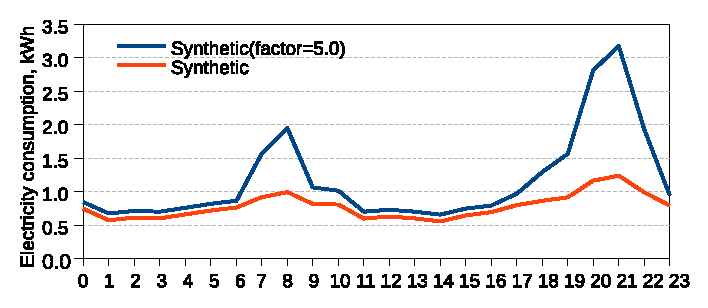
\includegraphics[scale=0.8]{images/onedayconsumptiondata}
\caption{Daily consumption profile}
\label{fig:onedayconsumptiondata} 
\end{figure*}

\begin{figure*}[t]
  \centering
  \subfigure[Empirical]{\label{fig:empricialdistribution}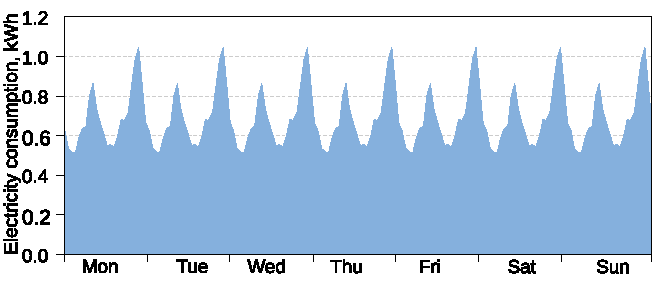
\includegraphics[scale=0.8]{images/empricialweeklyconsumptionpattern}}
  \subfigure[Synthetic]{\label{fig:syntheticdistribution}  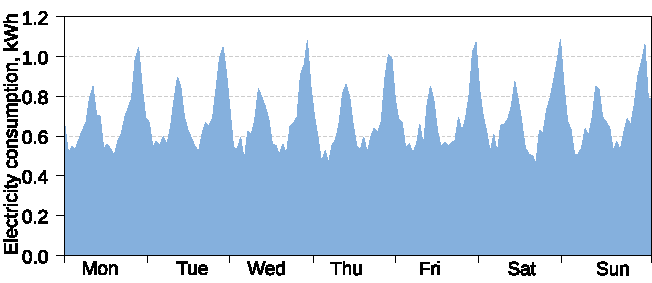
\includegraphics[scale=0.8]{images/syntheticweeklyconsumptionpattern}}
\caption{Weekly consumption pattern}
\label{fig:oneweekconsumptionpattern}
\end{figure*}

\begin{figure*}[htp]
  \centering
  \subfigure[Empirical]{\label{fig:empricialdistribution}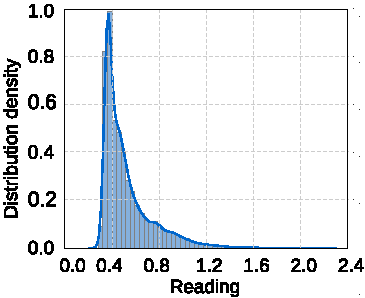
\includegraphics[scale=0.8]{images/empricialdistribution}}
  \subfigure[Synthetic]{\label{fig:syntheticdistribution}  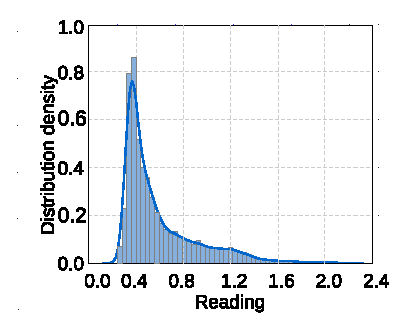
\includegraphics[scale=0.8]{images/syntheticdistribution}}
\caption{Distribution of hourly consumption of a customer}
\label{fig:distribution}
\end{figure*}


\begin{figure*}[htp]
  \centering
  \subfigure[Empirical]{\label{fig:empricialcentroid}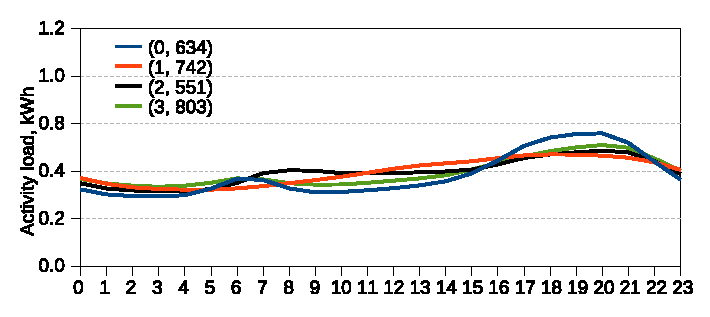
\includegraphics[scale=0.8]{images/empricialcentroid}}
  \subfigure[Synthetic]{\label{fig:syntheticcentroid}  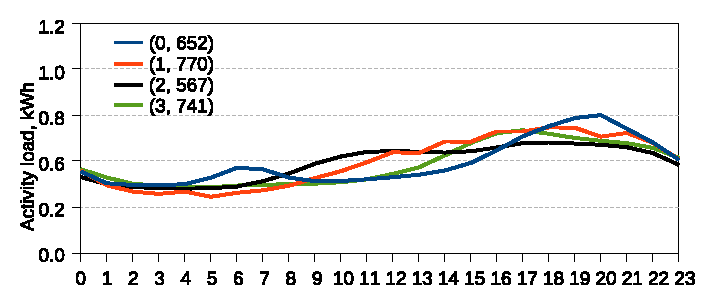
\includegraphics[scale=0.8]{images/syntheticcentroid}}
  \caption{Cluster centroids of daily activity load profiles}
\label{fig:centroids}
\end{figure*}

\begin{figure*}
  \centering
  \subfigure[With a fixed size of nodes, 16]{\label{fig:gensizeup}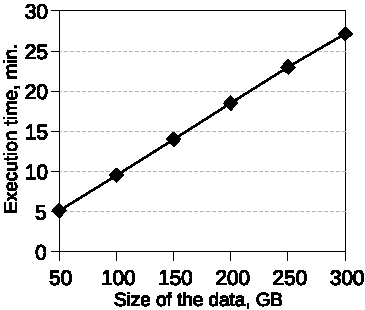
\includegraphics[scale=0.8]{images/gensizeup}}
  \subfigure[With a fixed size of data sets, 300GB]{\label{fig:genscaleup}  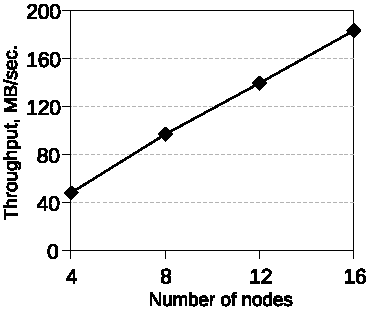
\includegraphics[scale=0.8]{images/genscaleup}}
\caption{Scalability of generating data}
\label{fig:centroids}
\end{figure*}

\raggedright
\flushleft
\begin{thebibliography}{20}



\end{thebibliography}
\end{document}
